Selleks et tõestada antud magistritöö eesmärki segmenteerida lageraie ja metsa alasi suurte visioonimudelitega, klusterdatakse DinoV2 väljundid, et leida, kas need alad on eristatavad. Selleks on vajalik eksperdiga valideerida ühe lageraie piirkonna alad, et kindel olla, et need vastavad tõele satelliidipildilt.

Joonisel \ref{fig:näidisSadeliidiPilt} on näidispilt eksperimendist, mille käigus püüti välja selgitada, kas mudelid suudavad eristada lageraie ja metsa alasid satelliidipiltidelt. Antud Sentinel-2 andmebaasist saadud pilt sai valitud esiteks sellepärast, et see on hea nähtavusega, võimalikult vähe pilvine ja soojemal hooajal, kui pole lund ja puud on lehteis. Teiseks on käesolev pilt heaks aluseks, sest sellel on sattunud raie- ja metsapiirkondi kõrvuti, mis võimaldab erinevatesse klassidesse kuuluvate alade üleminekukohti analüüsida.

\begin{figure}[H]
    \centering
    \includegraphics[width=.7\textwidth]{figures/seose_leidmine/näidisSadeliidiPilt.png}
    \caption{Näidis sateliidi pilt}
    \label{fig:näidisSadeliidiPilt}
\end{figure}

Joonisel \ref{fig:raieInfoMask} on näha lageraie piirkond, mis on toodud välja tumedama roosana, ja metsa piirkond, mis on joonisel heleroosana. Tegemist on aladega, mis on teada Keskkonnaametile ja mille kohta on olemas ka metsateatis. Satelliidipilt on saadud Sentinel-2 andmebaasist ja sellel on kümnemeetrine resolutsioon. Antud pilt on saadud raie teostamise ajast kuni 40 päeva hiljem, seega mahub õigesse ajaraamistikku, et piisavalt täpselt hinnata metsade seisukorda.

\begin{figure}[H]
    \centering
    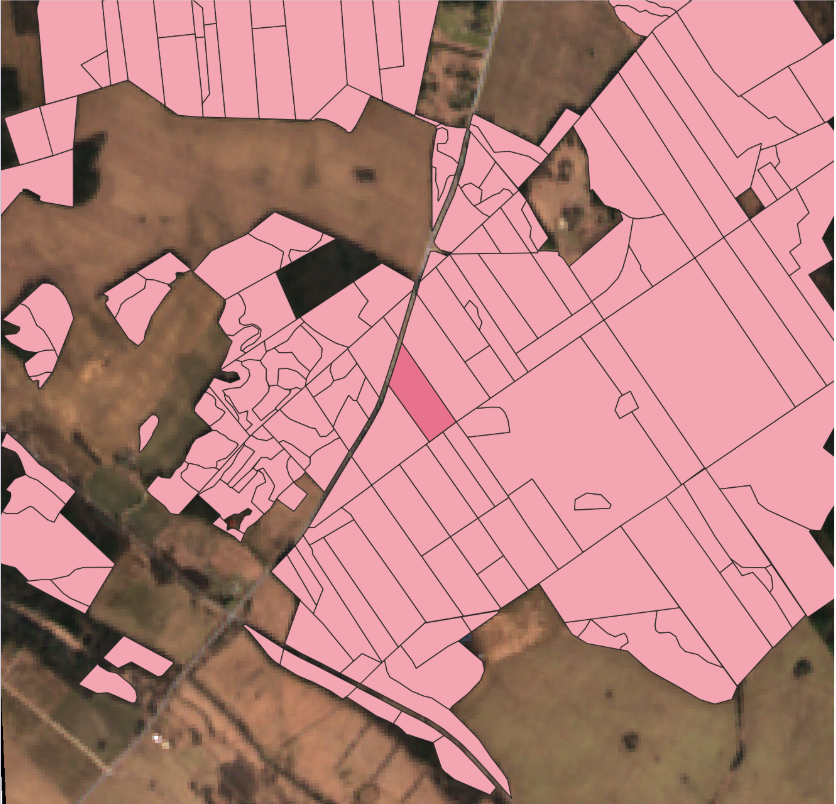
\includegraphics[width=.7\textwidth]{figures/seose_leidmine/raieInfoMask.png}
    \caption{Raie piirkonna mask sateliidi pildil}
    \label{fig:raieInfoMask}
\end{figure}

Joonisel \ref{fig:raieInfoMask_ekspert} on näha lageraie piirkond, mis on toodud välja tumepunasena ja metsa piirkond, mis on märgitud rohelisega. Ekspert on võtnud metsateatistest saadud info alade tuvastamisel aluseks, aga sellele lisaks kasutas ta ka muud teavet nagu ortofotosid ja erinevate lainepikkuste pilte, et leida täpsemad piirded metsade ja raiealade vahel. Ekspert on leidnud, et antud piirkonnas leidub alasid, mis ei vasta metsateatistes märgendatud infole. Näiteks on pildil alasid, mis teatistes on märgitud metsaks, aga silmaga vaadates kujutab hoopis raiet ja ka vastupidi. Seega on eksperdi poolt loodud mask palju täpsem ja seetõttu oli eksperdi kaasamine vajalik andmestiku loomise protsessis.

\begin{figure}[H]
    \centering
    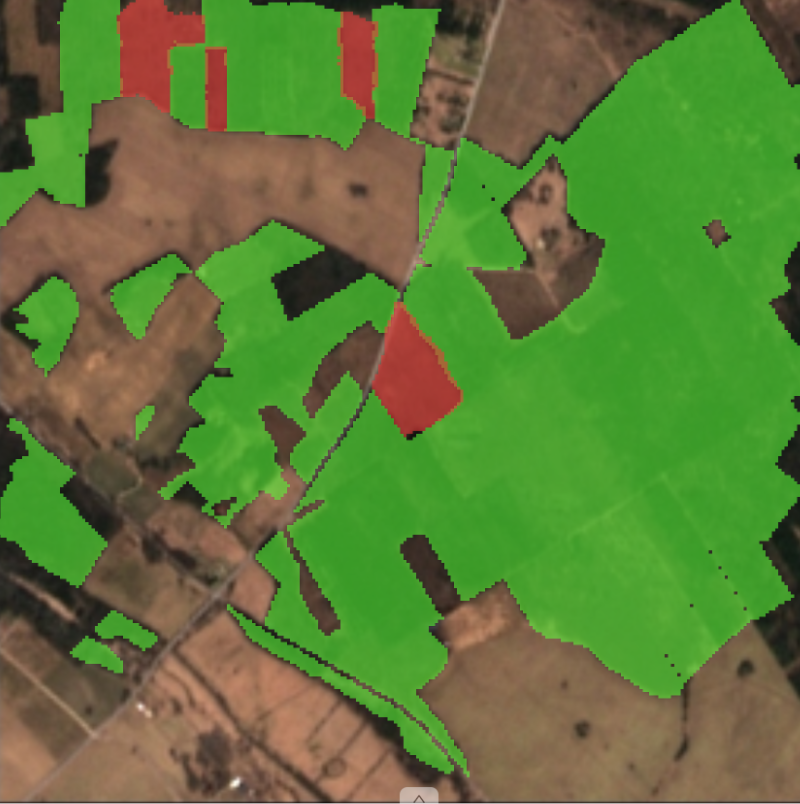
\includegraphics[width=.7\textwidth]{figures/seose_leidmine/raieInfoMask_ekspert.png}
    \caption{Raie piirkonna mask eksperdi poolt korrigeeritud}
    \label{fig:raieInfoMask_ekspert}
\end{figure}

Järgneval joonisel \ref{fig:segmenteeritudPealiskiht}, rakendati klastrianalüüsi süvaõppemudelist saadud
kõrgdimensionaalsetele tunnusevektoritele, mis esindavad sisendpildi
diskreetseid paiku. Eelkõige kasutati k-keskmise algoritmi, et grupeerida need
tunnusevektorid sarnaste semantiliste omaduste alusel. Igale pildilaigule vastav
tunnusevektor määrati ühte eelnevalt defineeritud arvu klastritesse, mille
tulemusena saadi diskreetne klastermärgis iga pildipaiga jaoks. Seejärel
visualiseeriti saadud klastermärgis pildil värvilise maskina, kus iga klaster on
esitatud unikaalse värviga, võimaldades seeläbi kvalitatiivselt hinnata mudeli
õpitud representatsioonide kohalikku sarnasust sisendpildil.

\begin{figure}[H]
    \centering
    \includegraphics[width=.7\textwidth]{figures/seose_leidmine/segmenteeritudNäidis.png}
    \caption{Segmenteeritud näidis sateliidi pildist}
    \label{fig:segmenteeritudPealiskiht}
\end{figure}

Joonisel \ref{fig:tsneDinoPatchEmbedings} on rakendatud klassipõhist klasterdamise meetodit, mille eesmärk on luua
pildimaterjalist semantiliselt sidusaid piirkondi, grupeerides pildi elemendid
eelnevalt defineeritud klassifikatsioonikategooriate alusel. Lähtudes mudeli
genereeritud klassifikatsiooniväljunditest, määratakse iga pildielement kõige
tõenäolisemasse klassi, mille alusel moodustatakse klastrid. Selle meetodi
rakendamise tulemusena saadakse segmentatsioon, kus ühte klastrisse kuuluvad
pildi osad on mudeli poolt klassifitseeritud sarnaselt. Lõppeesmärk on seeläbi
genereerida pildist arusaadavam representatsioon, mis
võimaldab interpreteerida pildi sisu semantilisel tasemel, tuues
esile objektide ja piirkondade klassipõhised seosed. Pildil on väljatoodud klass 1 mis on mets ja klass 2 mis on lageraie, lisaks sai eemaldatud tausta klass, et oleks kergem jälgida uuritavaid klasse.

\begin{figure}[H]
    \centering
    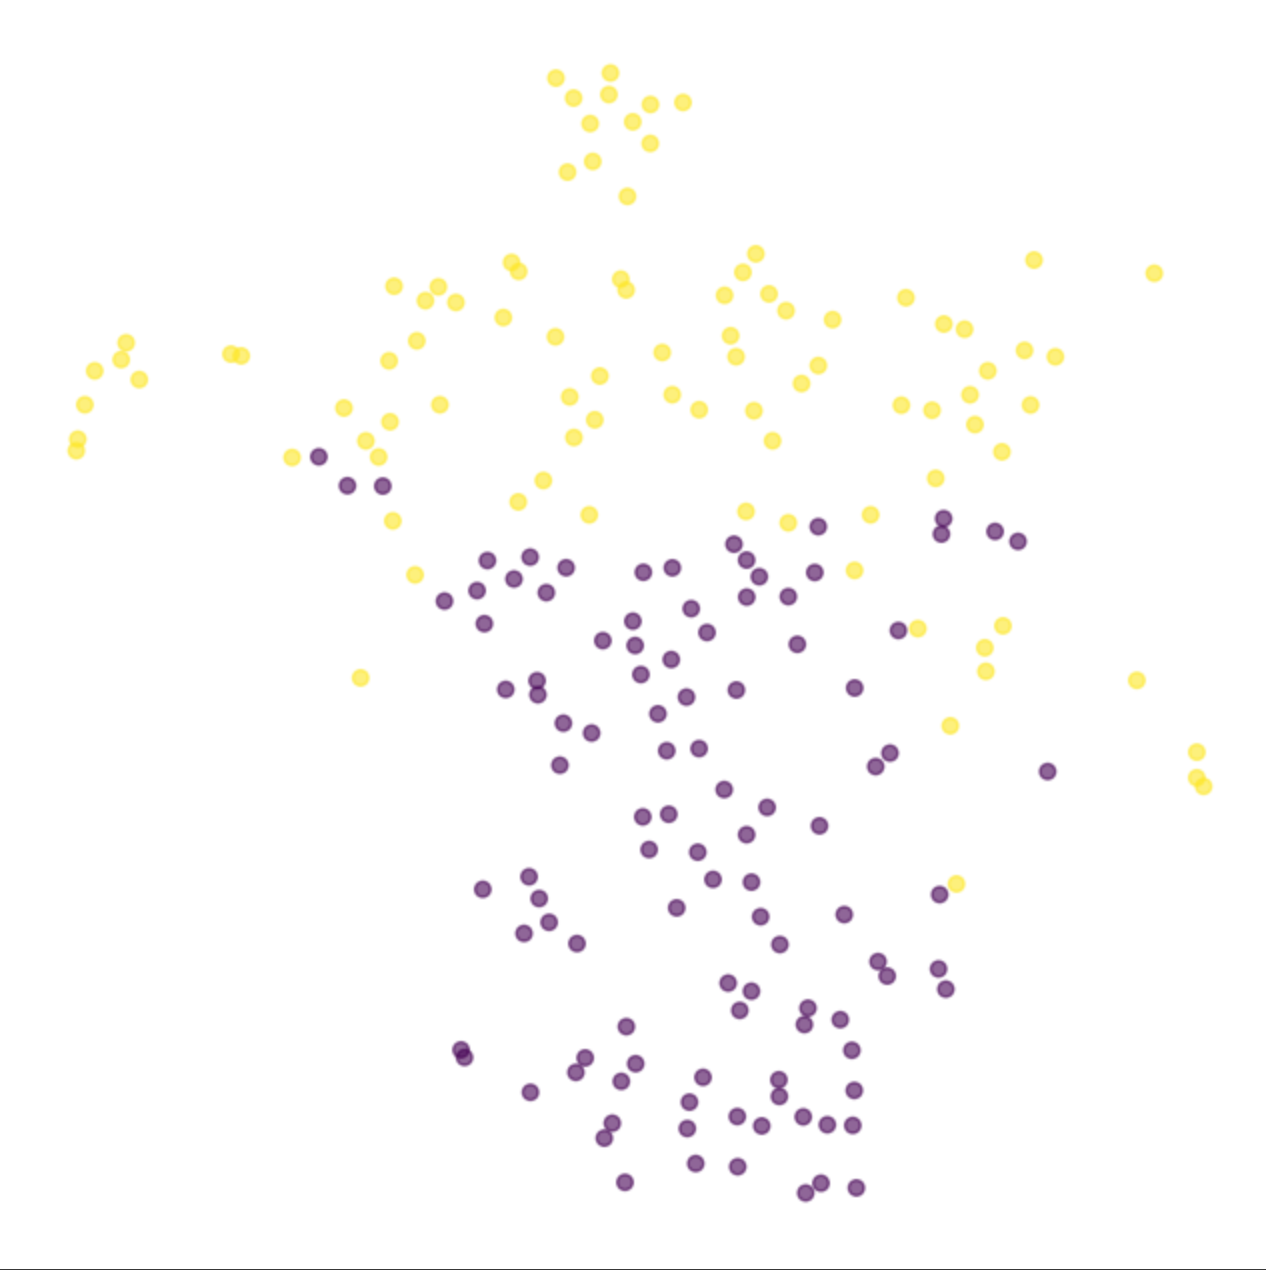
\includegraphics[width=.7\textwidth]{figures/seose_leidmine/tsneDinoPatchEmbedings.png}
    \caption{T-SNE kluster analüüs DinoV2 mudeli väljunditest}
    \caption*{kollane - mets, lilla - lageraie, roheline - taust}
    \label{fig:tsneDinoPatchEmbedings}
\end{figure}

Siit võis näha, et lageraie ja mets on eristatavad ja annavad alust edasi uurida, millised alusmudelid suudavad paremini eristada lageraie ja metsa alasid.
